\section{Cloud-native NFV}
Network virtualization and especially the switch from network functions residing inside purpose specific hardware towards VNFs, have been introduced in section \ref{sec:networkV}. The advantages are manifold, and include but are not limited to the following: Reduce the physical complexity of networks by eliminating the need for a majority of function-specific black boxes. This also causes a decline in setup and operational costs, since the highly specialized devices are expensive, consume more power and also require significant personel hours. This is mainly due to their vendor-specific functionality, and the need to physically install and configure them with limited possibilities of automation. Building new network services has become much easier and faster and can result in faster time to market while also ensuring higher return of investment. Reacting to fluctuating has become much easier and cost efficient. Finally, since the functionality is only bundled in software the emergence of ecosystems provide a more competitive market and favors innovative ideas. 

\subsection{NFV shortcomings}
This is definitely a step into the right direction towards a leaner and future proof network design. VNFs have been essential to redesigning networks and allowing for new use cases and business models. As much as this is a breakthrough, there are still some shortcomings of this approach that need to be considered. 

As previously explained, the main virtualization technique in VNFs has mainly been the virtual machine. Initially, the focus was on porting the functionality from a physical box into a virtual software artifact that runs inside a VM. The resulting functions are equally vertically integrated as their original, physical counterparts, following a rather monolithic approach. This has two main drawbacks:
First, the hypervisor-based virtualization is generally considered very resource heavy, due to inherent redundancy. On top of the host's infrastructure and operating system, a hypervisor orchestrates the the resource access of the guest's operating system (OS). Each instance of a VM on the same host has to rely on the hypervisor to get access to the resources that its OS can then use. 
Second, it is not enough to just port the VNF to use a container instead, the payoff would be minimal. Instead, the problem lies in the monolithic architecture of the function, which prevents a more flexible approach to service composition. Splitting up highly complex functions into logically separated, small and stateless components has multiple benefits, among which are more efficient resource utilization with much more appropriate scaling. Additionally, this allows for a more fine grained service composition and facilitating the development effort immensely by allowing for easier automation efforts. 

% NFV to microservices and containerization???
% Problems? Copy 1:1 hw appliance to vm, not efficient, throughput/all traffic guided through commodity hardware (-> dpdk) ; Added complexity! Placing functions? No autohealing, scaling, load-balancing, etc. Resilience? Fault-tolerance? Public vs Private cloud
%NFV and VNF basics \cite{mijumbi2016network} NFV real-world impact \cite{bilal2016impact} Service orchestration \cite{de2019network}


\subsection{Enabling Technologies and Concepts}
Mitigating the shortcomings of traditional VNFs can be realized by using specific technologies and adhering to cloud-native development principals. Such enabling technologies will be explored in the following.

\subsubsection{Docker}
Opposing the the concept of hypervisor-based virtualization is that of container-based virtualization which eliminates the need for a dedicated version of an OS with all its stack in each VM instance. It rather makes use of the host's kernel directly, circumventing a lot of the overhead a VM introduces. Figure \ref{fig:docker} shows the two approaches in contrast to each other. The most famous container project is called Docker. 

\begin{figure}[h]%
	\centering
	\subfloat[Hypervisor-based virtualization]{{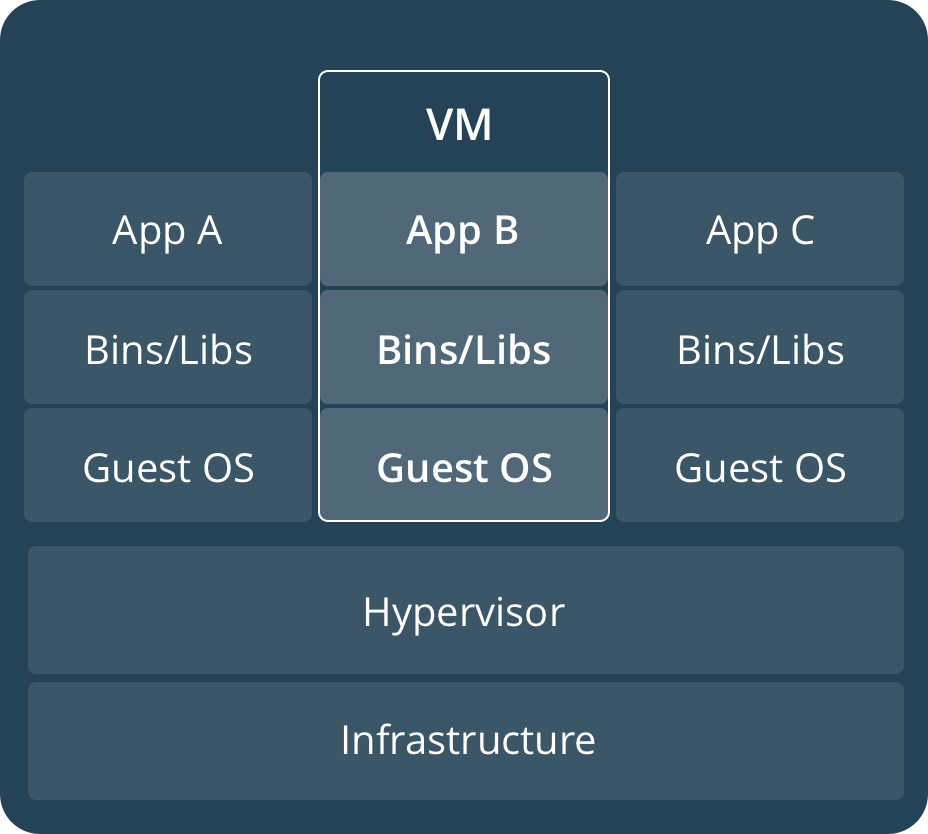
\includegraphics[width=.45\linewidth]{images/vm.png} }}%
	\quad
	\subfloat[Docker container]{{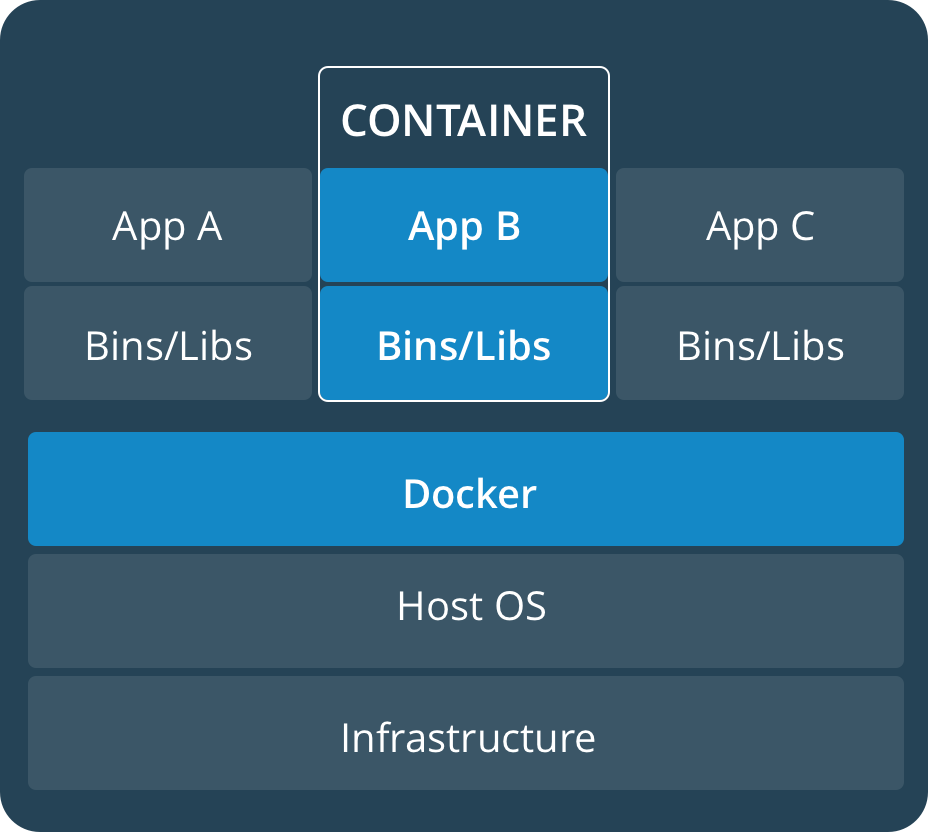
\includegraphics[width=.45\linewidth]{images/dockerContainer.png} }}%
	
	\caption{Comparison between hypervisor-based virtualization and Docker \cite{dockerdocu}}
	\label{fig:docker}
\end{figure}

It is an open source project that was originally build from many preexisting technologies in order to provide a more efficient virtualization technique as opposed to VMs. The tools that were used are mostly part of the Linux kernel as for example control groups (cgroups), used to manage and orchestrate the resource usage of a group of processes. Together with namespaces , that provide means to make resources only visible to a set of processes, they build the basis to separate the executable units from each other. These units are called \textit{containers} and are executed by the docker host via the system's kernel, using features like cgroups, namespaces, linux security models and many others to ensure strict separation from the rest of the system. Defining the composition and behavior of such a container is being done with so-called images. They are the blueprint, from which multiple containers can be derived from encapsulating the predefined contents inside multiple, read-only filesystem layers. Containers have a thin, writable layer at their disposal which is ephemeral. For persistence, volumes can be used to share data between the host and the container environment. The layering system in docker strives to minimize redundancies by sharing identical layers between multiple images, keeping the overall storage needs low \cite{fink2014docker} \cite{morabito2015hypervisors}.

Docker has gained a lot of popoularity over recent years and as an open source project, it has favored the creation of a large ecosystem around it. This makes the usage of docker much easier, since documentation, community help and tutorials are readily available. When packaging an application or a service inside an image, often dependencies and libraries need to be included. The large ecosystem makes this almost painless, since many, official and verified images already exist that can be used as a basis.

\subsubsection{OVS and OpenFlow}
Provisioning network functionality inside containers necessitates that the attachement of the containers to the rest of the network can be realized with as much automation as possible, and secondly with high performance. Attaching the containers to virtual switches is an essential step since these can guarantee both of these requirements. 

Open vSwitch is such a switch, using the Openflow protocol to be able to communicate with an SDN controller and thus provide programmability. Since Linux Kernel 3.3, it it comes bundled in it and provides multi layer switches and additional tools for a consistent setup, configuration and monitoring. The documentation provides insight into the authors' vision of what its main purpose is: Making networking easier in multi-server deployments that heavily rely on virtualization. In support of this high-reaching goal are several design characteristics: Making the migration of entities in the network as easy as possible is one of the core advantages of VNFs and CNFs and is realized by allowing the migration of configuration with the associated host. Supporting automation of the network is the fact that OVS holds the state in a database (OVSDB) while supporting triggering events remotely. OVS supports the idea of separating network traffic logically by tagging the packets. Finally, high performance during the interplay of hard- and software is guaranteed by allowing the forwarding path of the bridges to use the in-kernel datapath and directly communicating with the network interface cards (NIC). This also allows for simultaneous management of physical and software networking entities with teh same technology. 

Figure \ref{img:ovs} shows how the different components of OVS interact. The OVSDB is located at the user space level and stores all the information about the virtual switch. Its contents is accessible via the SDN controller in the network, or the ovs-server.
Realizing the actual switch is the ovs-vswitchd daemon, located in user space. Communication and manipulation is being realized via the OpenFlow protocol and the Southbound API of the SDN controller. 
\cite{openvswitch} \cite{pfaff2015design}. 

\begin{figure}[h]
	\centering
	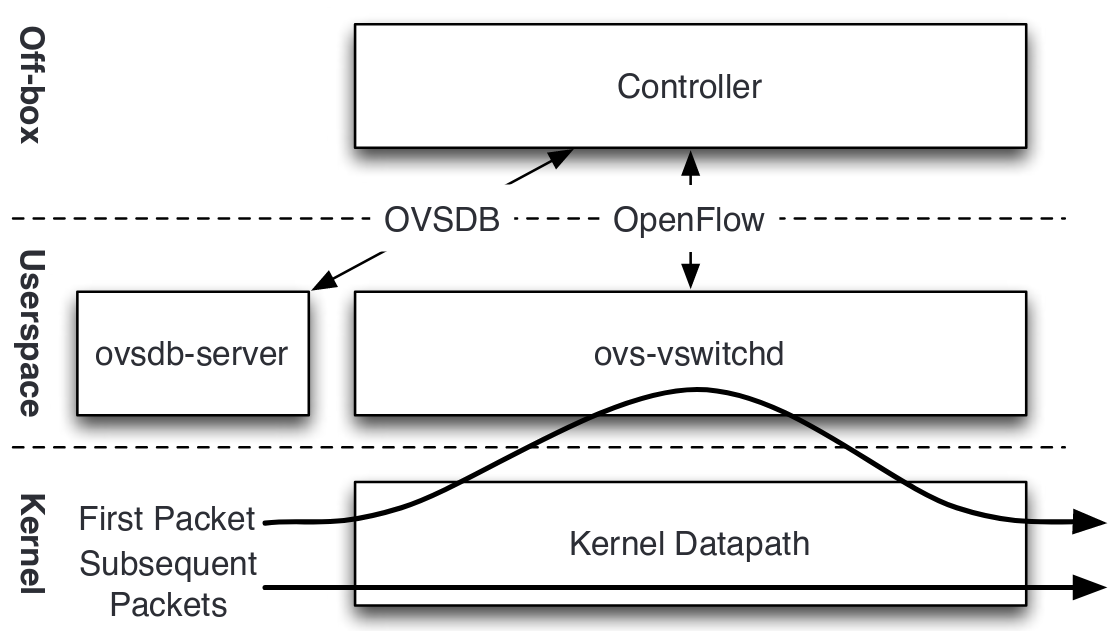
\includegraphics[width=1\linewidth]{images/openvswitch.png}
	\caption{Components and interfaces of Open vSwitch, source \cite{pfaff2015design}}
	\label{img:ovs}
\end{figure}

The OpenFlow protocol was developed in an educational environment by McKeown \textit{et al.} \cite{mckeown2008openflow} in 2008. Its main focus was to allow researchers to conduct experiments in their networks, while being "[...] open, vendor neutral, control-data plane interface [...]" \cite{berde2014onos}. Realizing its potential, the Open Networking Foundation (ONF) has adopted management and supports the extension and further development of OpenFlow.
In traditional forwarding switches packets are being registered from the ports they arrive, analyzed, and from the information in the packets' header specific rules for how to deal with them are learned. The inner workings of this behavior are transparent to the user without a possibility to modify or extend. In contrast, OpenFlow provides a possibility to manipulate so-called flow tables, that represent the rules of how to deal with incoming packets. 
Figure \ref{img:of} shows such a flow table that prescribes what to do with incoming packets as prescribed by the SDN controller. For each packet, a rule will be looked up from top to bottom which will prescribe the behavior exactly.  Information that can be used to match are various, like for example the MAC and IP addresses, port information and many others. In the figure these fields are marked in white color. The first column in grey prescribes what to do with a certain packet. For instance if a packet is destined to TCP port 25, it shall be dropped. Wildcards can be used and if nothing matches, the last line says to send the packet to the controller. Finally, the last column shows another advantage: Metrics for analysis of how often a rule has been applied. 
\cite{mckeown2008openflow}. 

\begin{figure}[h]
	\centering
	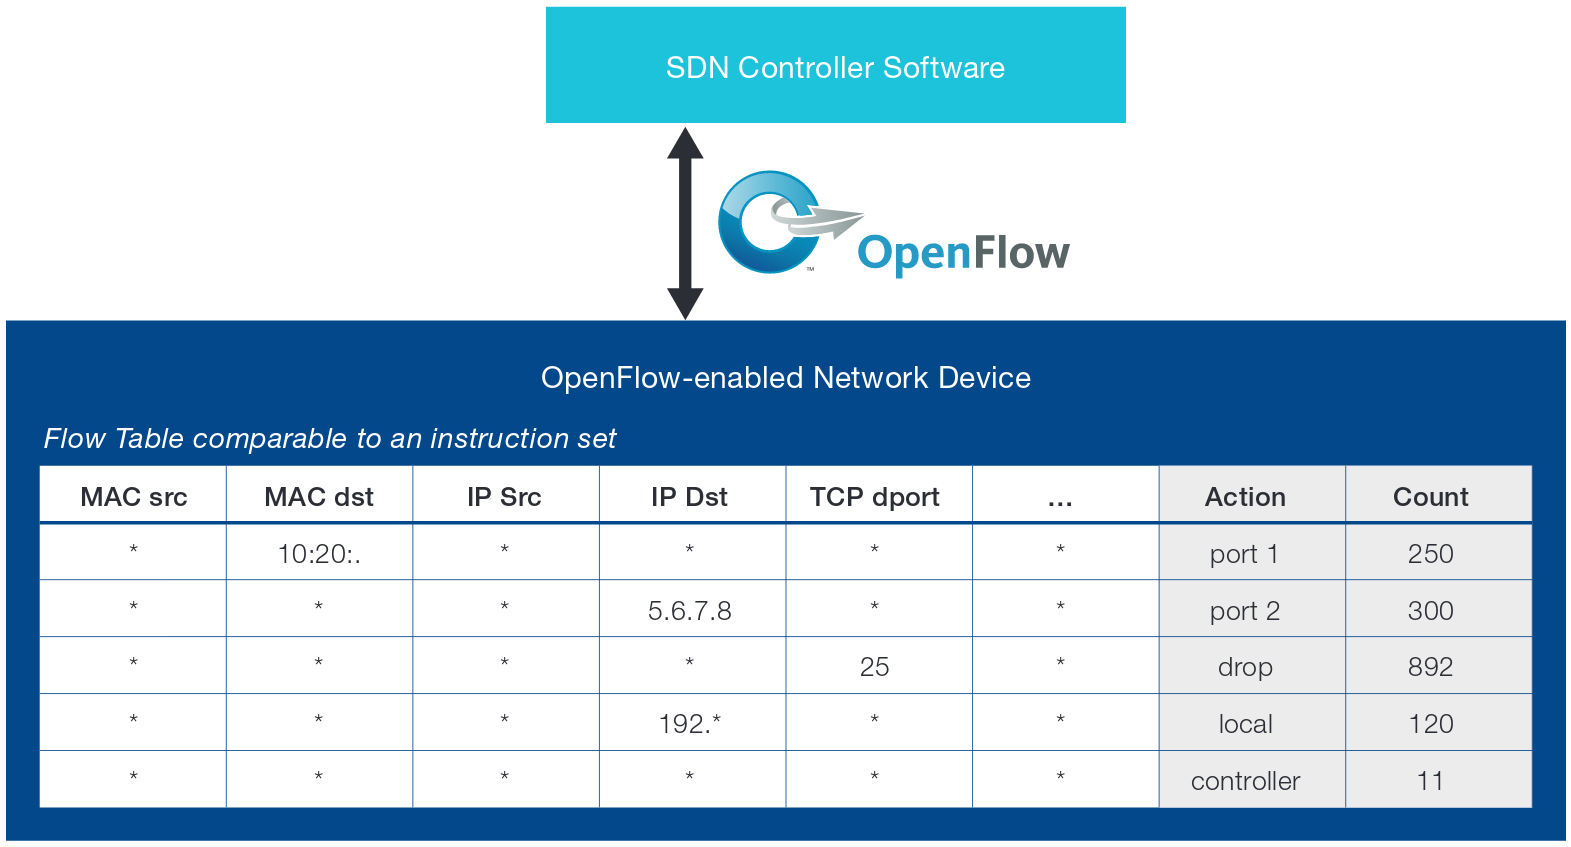
\includegraphics[width=1\linewidth]{images/of.png}
	\caption{Example of OpenFlow Instruction Set, source \cite{ofWhitePaper}}
	\label{img:of}
\end{figure}

This matching information can be manifold and includes but is not limited to the MAC/IP addresses of the sender or the receiver, the incoming port etc. In Figure \ref{img:of} these fields can be found on the left and are marked in white color. The two fields on the right serve a different purpose. The entry in the \textit{Action} column specifies what needs to be done to the packet if it conforms to the specified criteria. In this example it will either be output via port 1 or 2, dropped if it is directed at a TCP destination port 25, sent to local for processing if the IP destination starts with 192 or sent to the controller if no other rule applies. 

\subsubsection{Cloud-native paradigm}
OVS switches, SDN and Openflow allow for unprecedented possibilities to automate network setup and orchestration. 
\begin{figure}[h]
	\centering
	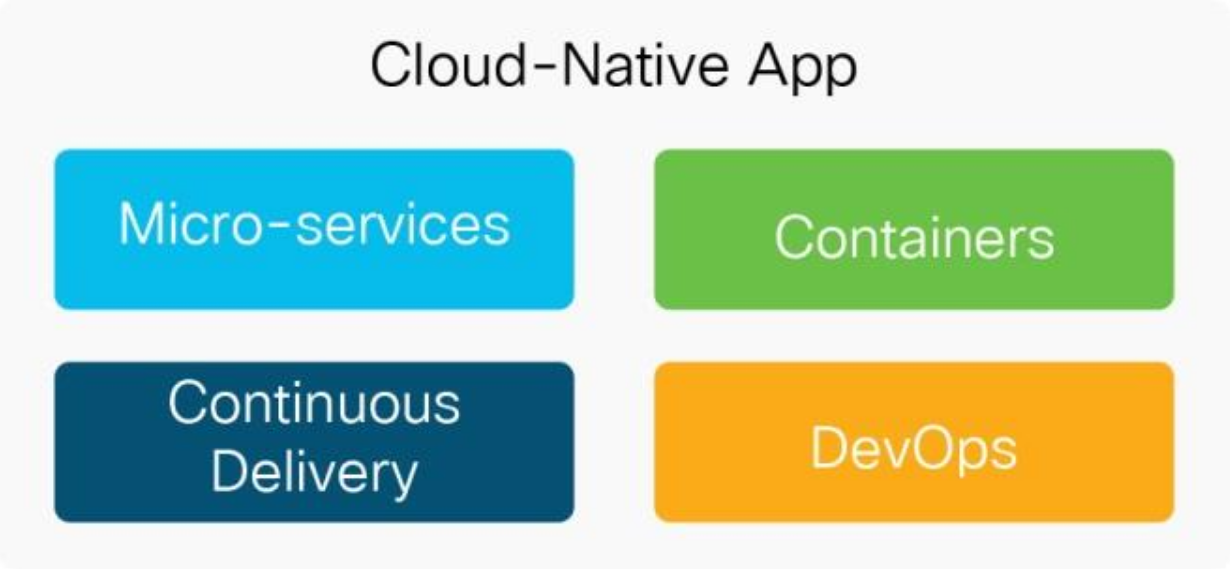
\includegraphics[width=0.75\linewidth]{images/cloudNativeApp.png}
	\caption{The principals of a cloud-native application as defined by the CNF \cite{CNF}}
	\label{img:cloudNativeApp}
\end{figure}

12 factor app


\subsubsection{Kubernetes}



%A lot of proprietary and custom build environments which VNFs are build for and deployed onto. This limits their effectiveness considerably.
%Virtual Machines, Openstack vs Docker and Kubernetes managing and orchestrating the deployment of network functionality, what are the benefits? What are drawbacks?
What is cloud-native, how do these principles relate to  the networking domain? Whitepapers published by Analysys Mason \cite{evolutionnfv} and Cisco \cite{CNF}



\subsection{CNFs}
Definition, advantages, state-of-the-art, testbed 

% Caveats: Mostly Cisco, lifecycle management, high-performance network, installation and operation


\begin{figure}
	\centering
	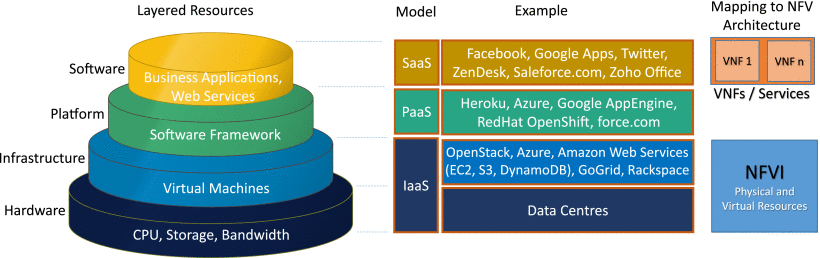
\includegraphics[width=1\linewidth]{images/arch.png}
	\caption{This is the caption \cite{mijumbi2016network}}
	\label{img:arch}
\end{figure}

